\begin{frame}[fragile]{GEANT4 Introduction}
What GEANT4 is:
\begin{itemize}
  \small
  \item \href{geant4.cern.ch}{geant4.cern.ch}
  \item Free software package for the simulation of the passage of particles through matter
  \item Essentially a collection of tools for geometry, materials, physics models, events and digitization, visualizations $\dots$
  \item Maintained by the CERN community, widely used in physics
\end{itemize}
What GEANT4 is not:
\begin{itemize}
  \small
  \item For the timid
  \begin{itemize}
    \item Users are responsible for correctly implementing their own physics
    \item Users are responsible for correctly implementing their own analysis
  \end{itemize}
  \item Stagnant - major release are still occurring
\end{itemize}
\hyperlink{G4Main}{\beamerbutton{Return to Energy Deposition}}
\hyperlink{toc}{\beamerbutton{Table of Contents}}
\end{frame}
%%%%%%%%%%%%%%%%%%%%%%%%%%%%%%%%%%%%%%%%%%%%%%%%%%%%%%%%%%%%%%%%%%%%%%%%%%
\begin{frame}[fragile]{Light Transport in GEANT4}
\begin{itemize}
  \item GEANT4 examples: \verb+ExampleN06+,\verb+extended/LXe+, \verb+extended/WLS+
  \item Sensitive detector on PMT
  \item Timing information
  \item Material Properties
  \small
  \begin{itemize}
    \item Optical absorption
    \item Index of refraction
    \item Surface properties - optical surface model \cite{5485130}
  \end{itemize}
\end{itemize}
\hyperlink{G4Main}{\beamerbutton{Return to Energy Deposition}}
\hyperlink{G4LightMain}{\beamerbutton{Return to Light Transport}}
\hyperlink{toc}{\beamerbutton{Table of Contents}}
\end{frame}
%%%%%%%%%%%%%%%%%%%%%%%%%%%%%%%%%%%%%%%%%%%%%%%%%%%%%%%%%%%%%%%%%%%%%%%%%%
\begin{frame}{Energy Deposition Spectral Validation}
  \begin{itemize}
    \item The energy deposition of thin films was calculated and compared to measurments
    \item Spectral shapes and average values were compared
  \end{itemize}
  \begin{columns}[onlytextwidth]
  \begin{column}{0.45\textwidth}
    \centering
    \begin{figure}
    	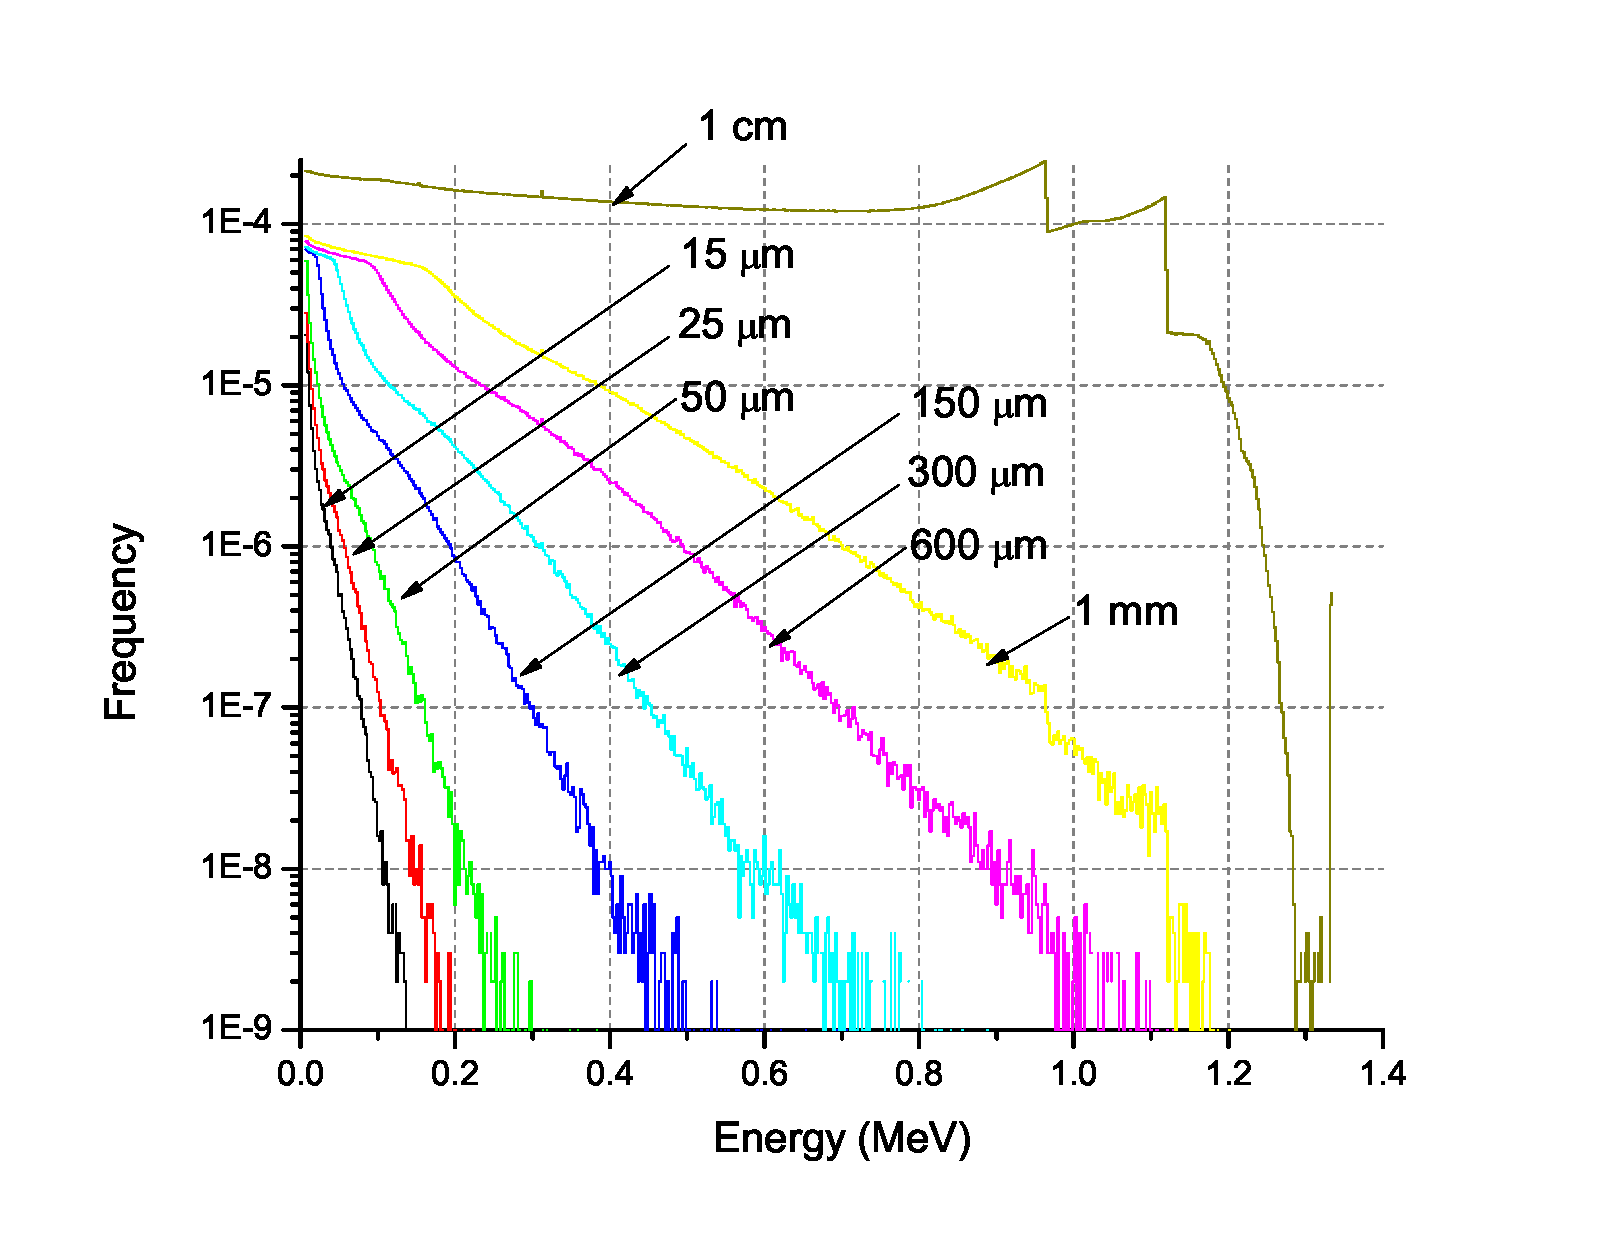
\includegraphics[width=\textwidth]{PS_EDepSim_Co60}
      \caption{Simulated}
    \end{figure}
  \end{column}
  \begin{column}{0.45\textwidth}
    \centering
    \begin{figure}
   	  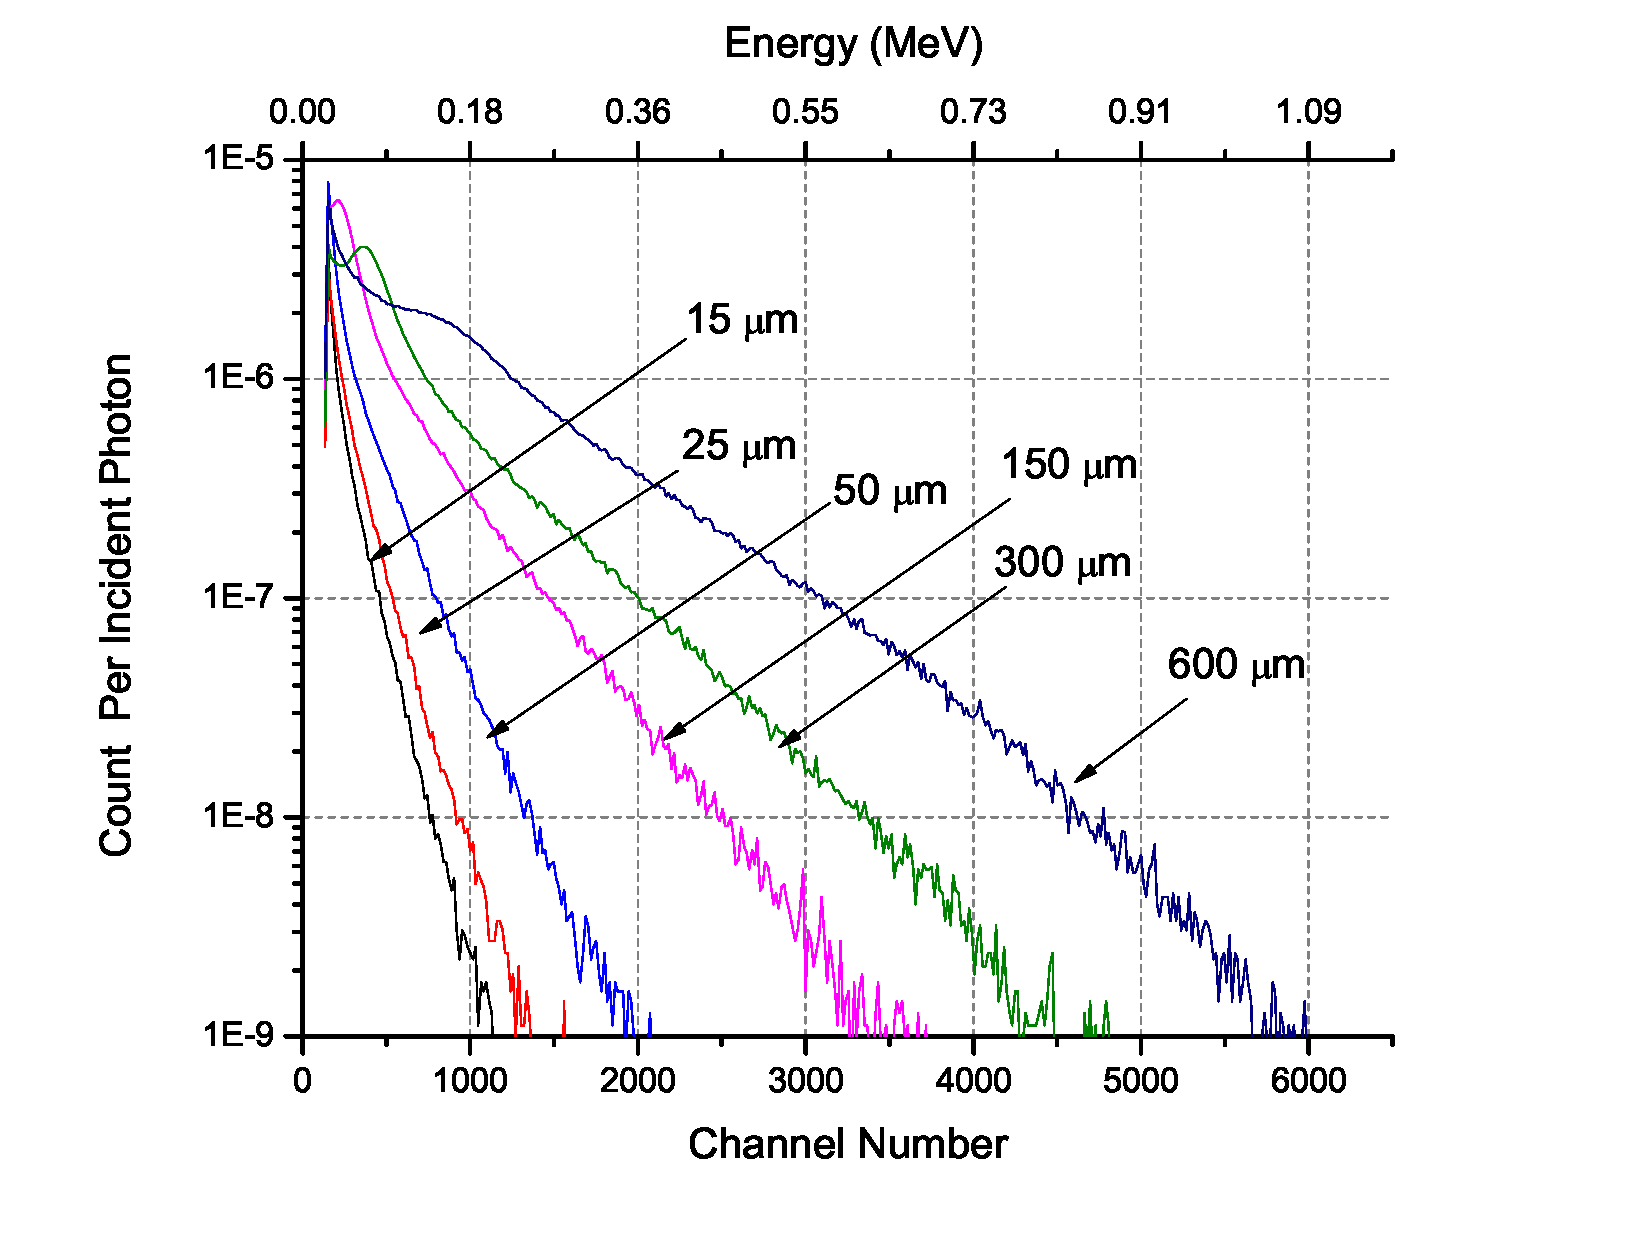
\includegraphics[width=\textwidth]{PS_GammaCR-Binned-FluxNorm_20LiF_5PPO}
      \caption{Simulated}
    \end{figure}
  \end{column}
  \end{columns}
\hyperlink{G4Main}{\beamerbutton{Return to Energy Deposition}}
\hyperlink{toc}{\beamerbutton{Table of Contents}}
\end{frame}
%%%%%%%%%%%%%%%%%%%%%%%%%%%%%%%%%%%%%%%%%%%%%%%%%%%%%%%%%%%%%%%%%%%%%%%%%%
\begin{frame}[fragile]{Optical Material Properties}
Most difficult part of simulation is correct properties
\begin{lstlisting}
void Materials::SetOpticalPropertiesGS20(){
    // Index of Reflection (146 nm to 1570 nm)
    const G4int nRINDEX = 13;
    G4double photonEnergyRINDEX[nRINDEX] = 
    {8.550*eV,4.723*eV,3.262*eV,2.492*eV,2.016*eV,
    1.692*eV,1.458*eV,1.281*eV,1.142*eV,1.031*eV, 
    0.939*eV,0.862*eV,0.797*eV};
    G4double RefractiveIndexGlass[nRINDEX]=
    {1.6508,1.5266,1.4980,1.4872,1.4819,    
    1.4790,1.4772,1.4760,1.4752,1.4746,    
    1.4742,1.4738,1.4736};
    // Absorbition Length
    const G4int nABS=2;
    G4double photonEnergyABS[nABS] = {3.5*eV,1.75*eV};
    G4double AbsLengthGlass[nABS] = {70*cm, 70*cm};  
\end{lstlisting}
\hyperlink{G4LightMain}{\beamerbutton{Return to Light Transport}}
\hyperlink{toc}{\beamerbutton{Table of Contents}}
\end{frame}
%%%%%%%%%%%%%%%%%%%%%%%%%%%%%%%%%%%%%%%%%%%%%%%%%%%%%%%%%%%%%%%%%%%%%%%%%%
\begin{frame}[fragile]{Optical Material Properties}
\begin{lstlisting}
    G4double photonEnergyEM[nEM] = {3.8,3.5,3.1,2.8,2.5};
    G4double emGS20[nEM]={0,0.19,0.37,0.32,0.10,0.02};
    MPTGS20->AddProperty("RINDEX",photonEnergyRINDEX,RefractiveIndexGlass,nRINDEX);
    MPTGS20->AddProperty("ABSLENGTH",photonEnergyABS,AbsLengthGlass,nABS);
	  MPTGS20->AddProperty("FASTCOMPONENT",photonEnergyEM,emGS20,nEM);
    MPTGS20->AddConstProperty("FASTTIMECONSTANT",50*ns);
    MPTGS20->AddConstProperty("SCINTILLATIONYIELD", 3600*MeV);
    MPTGS20->AddConstProperty("YIELDRATIO", 1.0);
    MPTGS20->AddConstProperty("RESOLUTIONSCALE", 1.0);
}
\end{lstlisting}
\hyperlink{G4LightMain}{\beamerbutton{Return to Light Transport}}
\hyperlink{toc}{\beamerbutton{Table of Contents}}
\end{frame}
%%%%%%%%%%%%%%%%%%%%%%%%%%%%%%%%%%%%%%%%%%%%%%%%%%%%%%%%%%%%%%%%%%%%%%%%%%
